\documentclass{beamer}
\usetheme{CENIDETDIE}
\setbeamertemplate{caption}[numbered]
\usefonttheme[onlymath]{serif}

% ------------------------------------------------------------------------------------------------

\usepackage[utf8]{inputenc}
\usepackage[T1]{fontenc}
\usepackage{helvet}
\usepackage{graphicx} % Allows including images
\usepackage{booktabs} % Allows the use of \toprule, \midrule and \bottomrule tables
\usepackage{amsmath}
\usepackage{color}
\usepackage{hyperref}
%\usepackage{showframe}
\usepackage[absolute,overlay]{textpos} %To place the images
\usepackage[document]{ragged2e}
%\usepackage{authblk} %many authors
%\numberwithin{figure}{section}
%\usepackage{ragged2e}%To use justify
%\numberwithin{equation}{section}
%\usepackage{natbib}
\usepackage{multirow}
%\usepackage{apalike}
\usepackage{biblatex}
\addbibresource{references.bib}
%\usepackage[bottom]{footmisc}
%\usepackage[colorinlistoftodos]{todonotes}
\usepackage{graphicx}
\usepackage{caption}
\usepackage{subcaption}
% ------------------------------------------------------------------------------------------------
\title{\textbf{ \textit{Simplest Fermion Vector-Like Portal Dark Matter model:}}}
\subtitle{{\small 	Search in the compressed mass region at the CMS experiment}}
\author[C.Salazar]{\textbf{Camilo Salazar} }
\institute[UdeA]{camilo.salazar@cern.ch}

%\author{\textit{\textbf{Camilo A Salazar G}}}
%\institute{\url{camilo.salazar@cern.ch} }
\date{\today}


% ------------------------------------------------------------------------------------------------

\begin{document}

% ------------------------------------------------------------------------------------------------

\begin{frame}[plain,t]
\titlepage
\end{frame}


% ------------------------------------------------------------------------------------------------

\begin{frame}[plain,noframenumbering]
  \addtocounter{framenumber}{-1}
  \scriptsize
%   \thispagestyle{empty}
  \frametitle{Contenido}
  \setbeamertemplate{section in toc}[sections numbered]
  \tableofcontents[hideallsubsections]
\end{frame}

% ------------------------------------------------------------------------------------------------

\section{Introduction}
\begin{frame}
\frametitle{Introduction}
\justifying{
	
	
	Dark Matter (DM) constitutes one of the main unsolved problems in fundamental physics. 
	Ever since it was proposed to explain the rotation curves of galaxies, 
	some other astronomical observations left little doubt of its existence.
	\vspace{5 mm}
	
	Whatever DM is, the Standard Model (SM) is not able to produce a candidate that have, at the present time in 
	the universe, stability and also interact very little or not at all with known matter, proven properties of DM. 

}


\end{frame}

% ------------------------------------------------------------------------------------------------

\begin{frame}
\frametitle{Rotational Velocities}


\begin{figure}[!tbp]
	\centering
	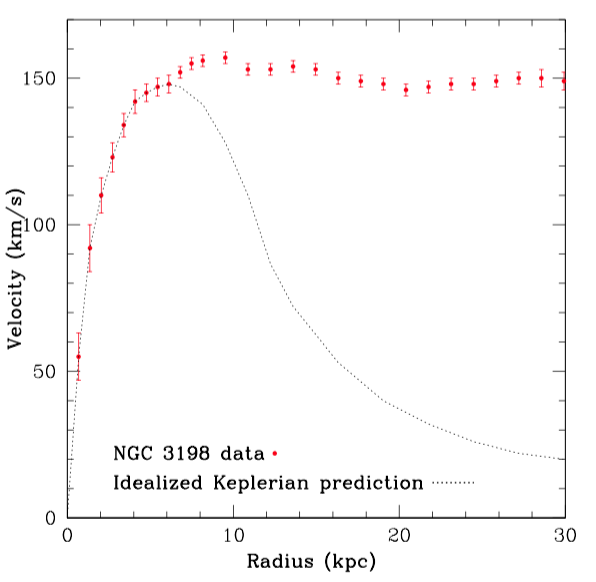
\includegraphics[width=0.6\textwidth]{pictures/fig_Introduction_rotation_curve_1}\label{fig:f1}
	\caption{Measured rotational velocities of HI regions in NGC 3198 compared to an idealized Keplerian behavior [Astron. and Astrophys. 223, 47-60]}
\end{figure}

\end{frame}

% ------------------------------------------------------------------------------------------------

\begin{frame}
\frametitle{Bullet cluster}


\begin{figure}[!tbp]
	\centering
	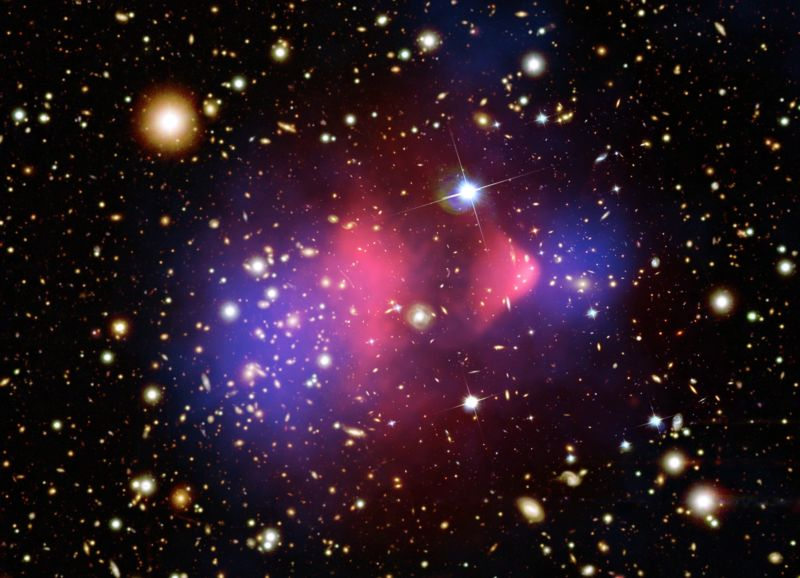
\includegraphics[width=0.8\textwidth]{pictures/bulletcluster}\label{fig:f2}
	\caption{The Bullet cluster, the result of a subcluster (the “bullet”) colliding with the larger galaxy cluster 1E 0657-56  [arXiv:1711.02117]}
\end{figure}

\end{frame}

% ------------------------------------------------------------------------------------------------


\section{Motivation}
\begin{frame}
\frametitle{Motivation}

\begin{figure}[!tbp]
	\centering
	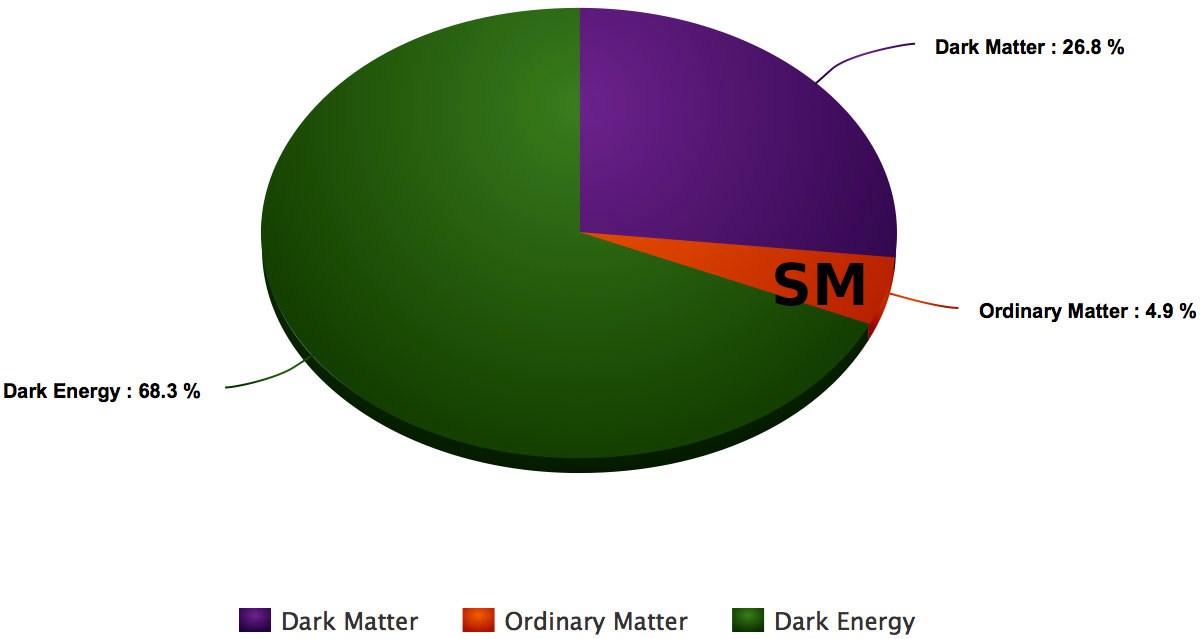
\includegraphics[width=0.9\textwidth]{pictures/pie}\label{fig3}
	\caption{{\scriptsize Simplified plot showing the estimate abundances}}
	
\end{figure}

\end{frame}

% ------------------------------------------------------------------------------------------------

\begin{frame}
\frametitle{Detection Channels}

\begin{figure}[!tbp]
	\centering
	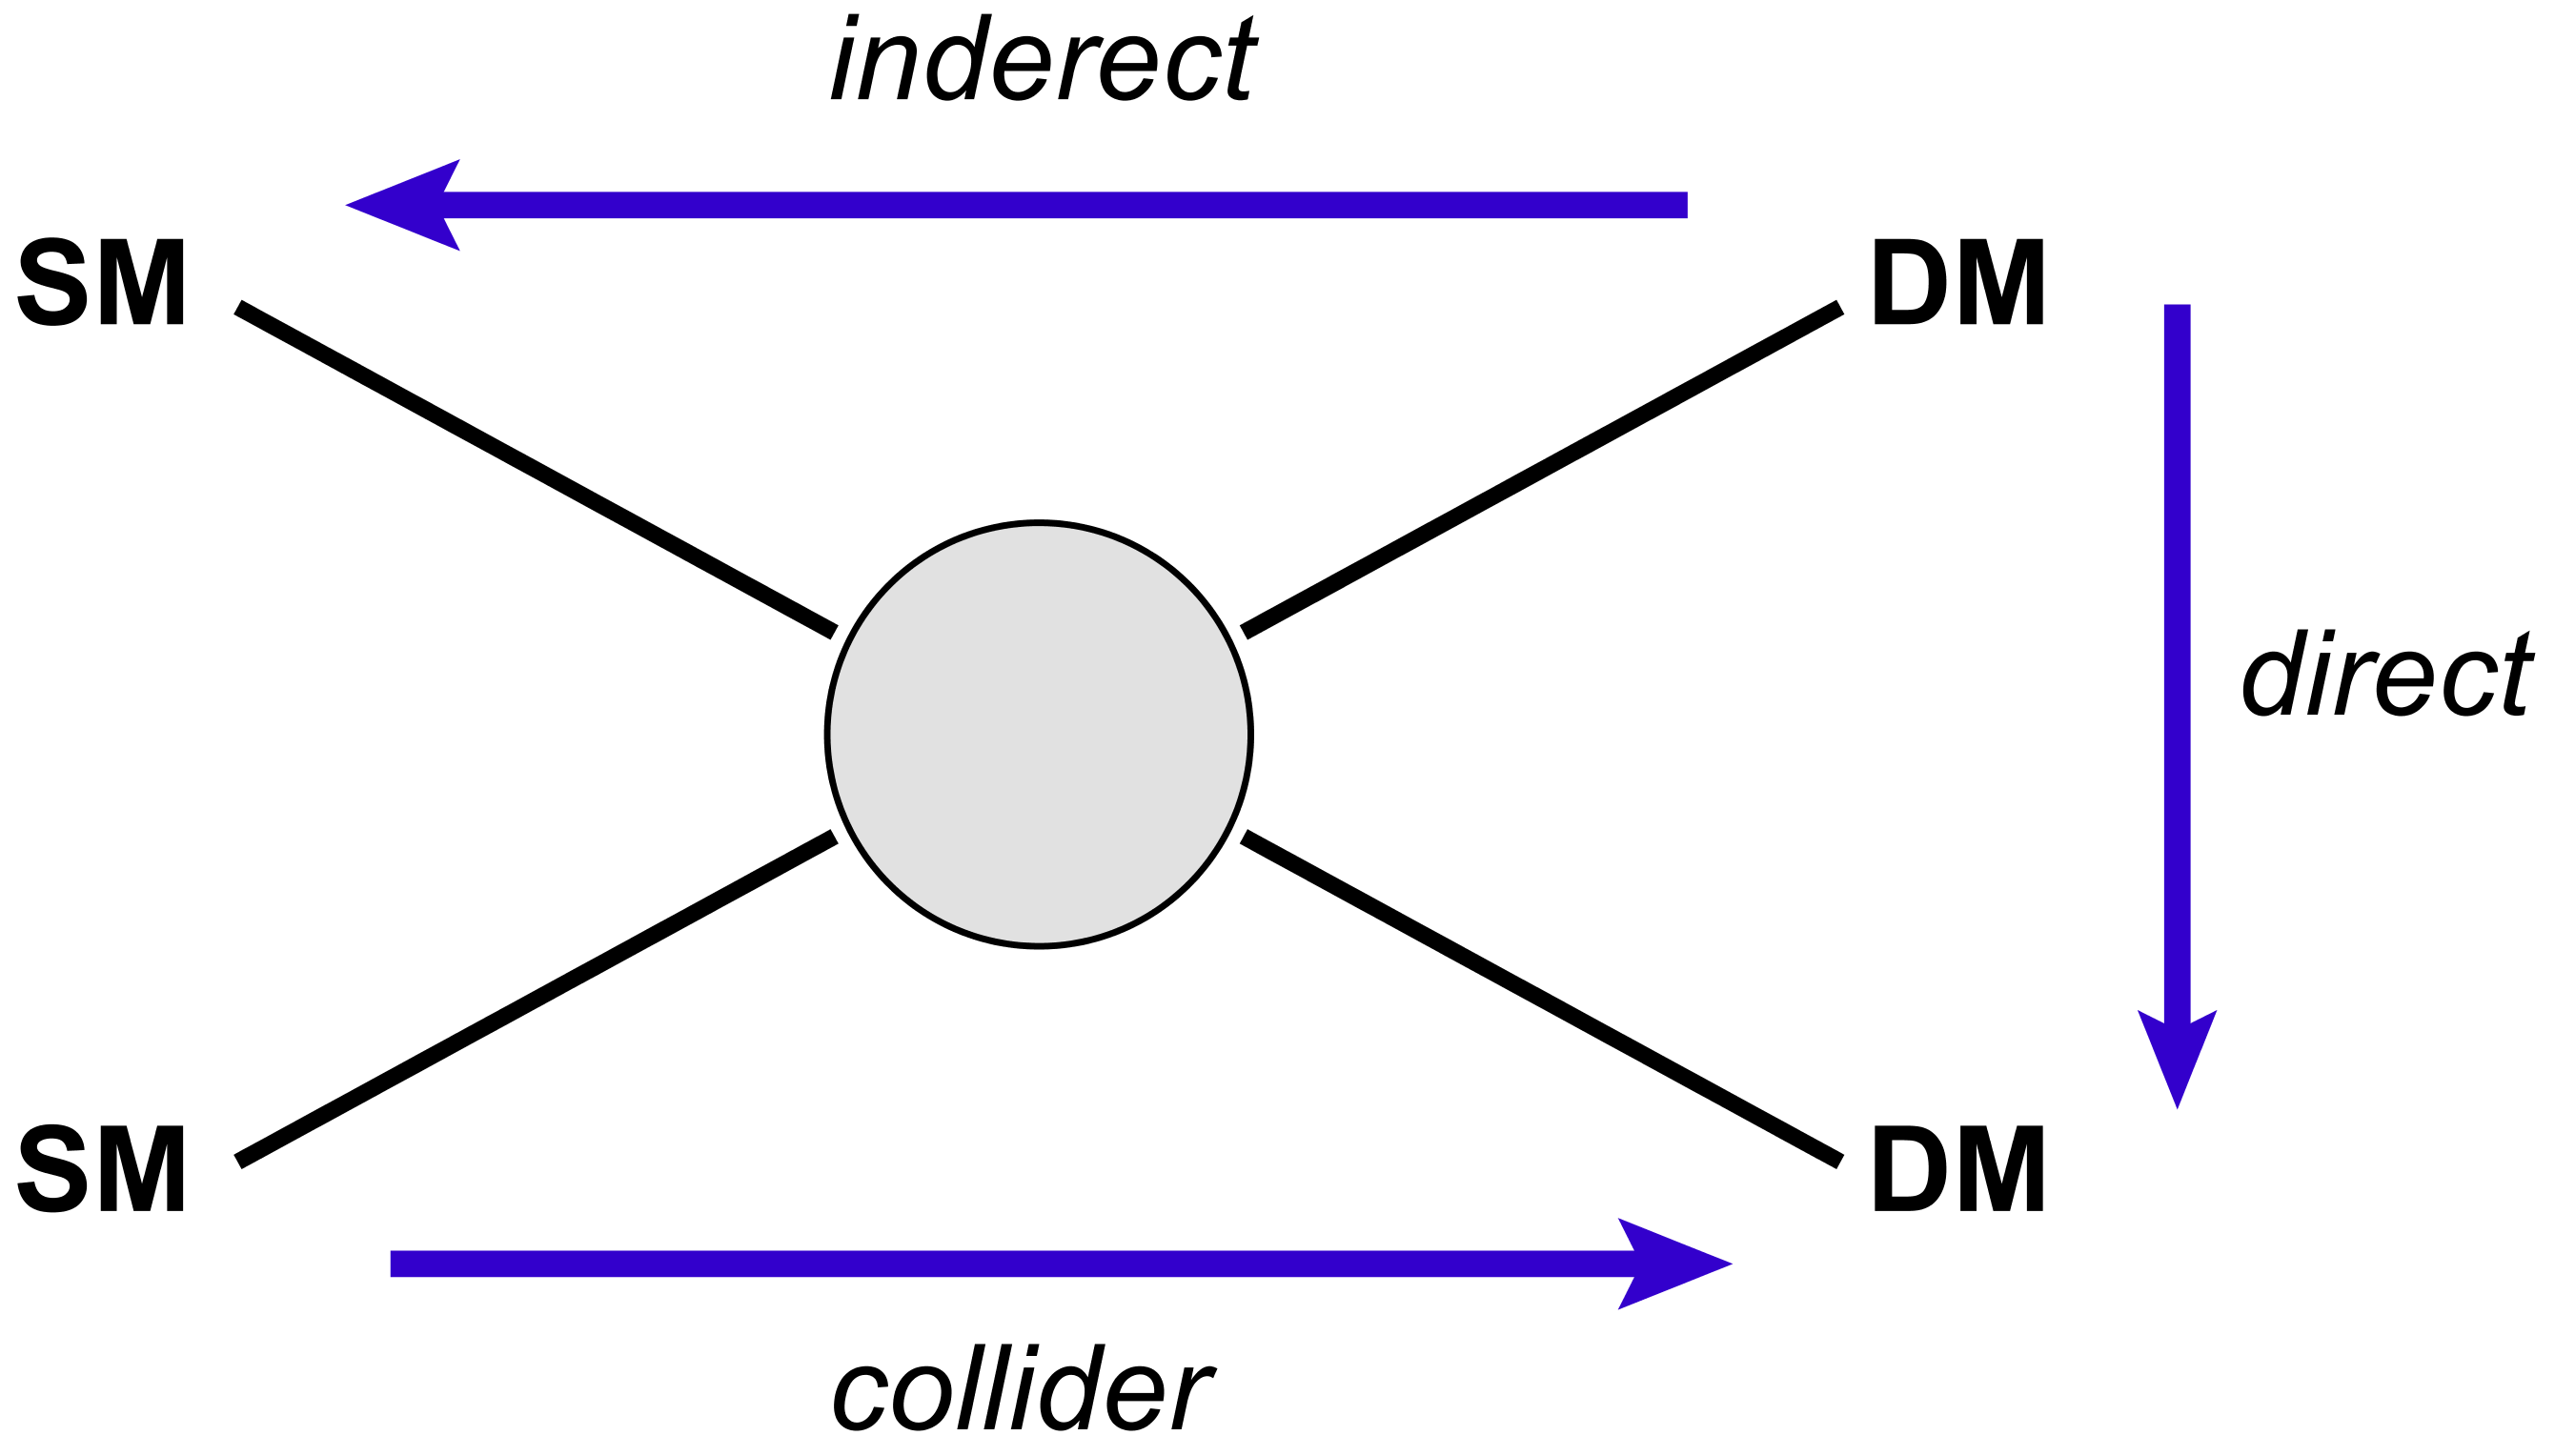
\includegraphics[width=0.9\textwidth]{pictures/Schem}\label{fig4}
	\caption{{\scriptsize Schematic showing the possible dark matter detection channels.}}
	
\end{figure}

\end{frame}
% ------------------------------------------------------------------------------------------------

%\begin{frame}
%\frametitle{Constrains Direct Detection}

%\begin{figure}[!tbp]
%	\centering
%	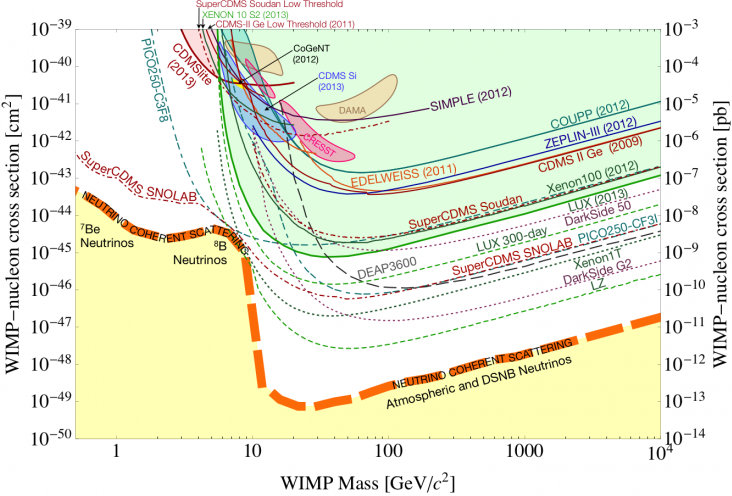
\includegraphics[width=0.9\textwidth]{pictures/WIPMS}\label{fig:f1}
%	\caption{{\scriptsize The predicted WIMP-nucleon scattering cross section as a function of WIMP mass.[APS Physics 6, 136] }}
	
%\end{figure}

%\end{frame}

% ------------------------------------------------------------------------------------------------

\section{Model}
\begin{frame}
\frametitle{Model}
 The VLF model introduce a vector-like charged fermion also $SU(2)_L$ singlet, and a scalar particle. The free Lagrangian reads
 \begin{equation}\nonumber
 \mathcal{L} = \mathcal{L}_{SM} +  m_F \bar{F}F + ( Y_\ell S \bar{F}\ell_R + {\rm h.c.} ) + V(S,H)~;
 \end{equation}\label{EQ}
 
 $m_F$ is the singlet fermion mass parameter, $\ell_R$ are the SM right-handed lepton fields, $Y_\ell$ 
 are the Yukawa couplings. 
 
 The contribution to the scalar potential is given by
 
 \begin{equation}\nonumber
 V(S,H) = \frac{m_S^2}{2} S^2 + \frac{\lambda_S}{4} S^4 + \lambda_{SH} S^2|H|^2 ~,
 \end{equation}
 
 with scalar mass parameter $m_S$ and quartic couplings $\lambda_{S}$ and $\lambda_{SH}$.
 


\end{frame}
% ------------------------------------------------------------------------------------------------
% ------------------------------------------------------------------------------------------------
\begin{frame}
\frametitle{Kinetic Lagrangian}

\begin{textblock*}{0.5\linewidth}(0.75\linewidth,0.2\linewidth) % {block width} (coords)
	
	\begin{figure}[!tbp]
		\centering
		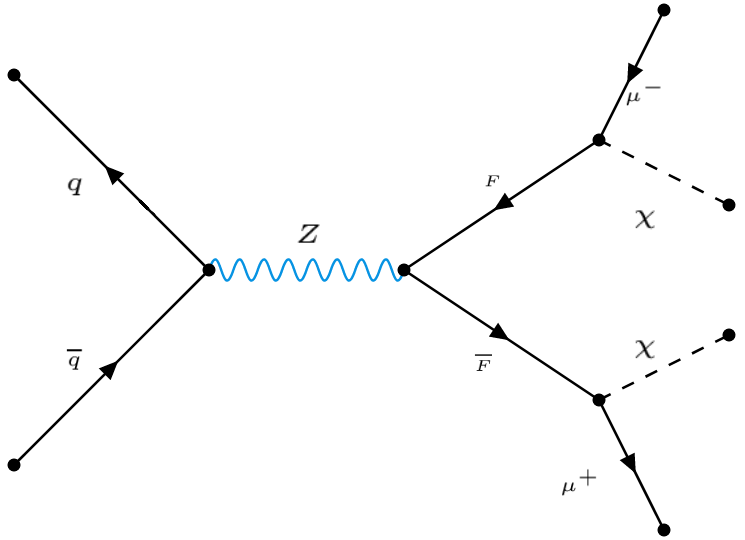
\includegraphics[width=1\textwidth]{pictures/DYVLFNoJet}
		\caption{{\scriptsize Pair-production of vector-like fermions ($p p \to F^- F^+ $),
				in a Drell-Yan process, followed by their decay into a lepton and the DM particle ($F^- \to \ell^- S +\rm{\ h.c.},\ \ell=e,\mu,\tau$ )}}
		\label{TowFerminon}
	\end{figure}
\end{textblock*}

\begin{textblock*}{0.46 \linewidth}(0.25\linewidth,0.25\linewidth) % {block width} (coords)
	{\small \justifying{
			
			The kinetic terms for thevector-like charged fermion reads as follows
			\begin{equation}
			\mathcal{L} ~ \bar{F}(D_{\mu}\gamma^{\mu})F,
			\end{equation}
			
			consequently the simplest production and decay process at the LHC
			is pair-production of vector-like fermions,
			followed by their subsequent decay to a lepton and the DM scalar.
					
			
	}}
\end{textblock*}

\end{frame}
% ------------------------------------------------------------------------------------------------
% ------------------------------------------------------------------------------------------------

\begin{frame}
\frametitle{Model}

\begin{textblock*}{1\linewidth}(0.25\linewidth,0.25\linewidth) % {block width} (coords)
	\justifying{

	We focus on scenarios where the vector-like portal for DM annihilation is dominant and, therefore, we set initially.
	\begin{equation}\nonumber
	\lambda_{SH}=0;
	\end{equation}
	 
	also we assume that the DM candidate does not couples to the electron.
	\begin{equation}\nonumber
	Y_{e}=0;
	\end{equation}
	
	the remaining parameters, $Y_{\mu}$,$Y_{\tau}$ ,  $m_S$ and  $m_F$ are allowed to vary freely.
	
	Also we are searching into the compress mass regime 
	
		\begin{equation}\nonumber
		 \Delta m=m_{F}-m_S\lesssim 50\ \text{GeV}
		\end{equation}
	}
\end{textblock*}

\end{frame}

% ------------------------------------------------------------------------------------------------

%\begin{frame}
%\frametitle{Creation of DM in the Early Universe}

%\begin{figure}[!tbp]
%	\centering
%	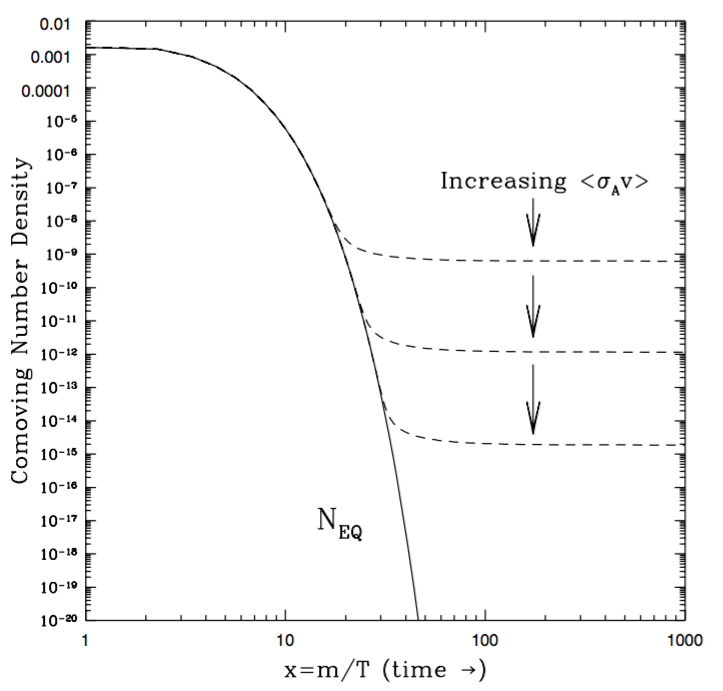
\includegraphics[width=0.7\textwidth]{pictures/FrizzOut}\label{fig2}
%	\caption{{\scriptsize Equilibrium (solid curve) and relic abundance (dashed curve) of WIMP particles. Figure is taken from 	arXiv:hep-ph/9506380}}
%	
%\end{figure}

%\end{frame}
% ------------------------------------------------------------------------------------------------

\section{Collider searches for DM}
\begin{frame}
\frametitle{Collider searches for DM}

\begin{alertblock}{Signals}
	\begin{enumerate}
		\item Cascades of heavier particles to the DM candidate and SM.
		\item[]
		\item DM production in association with other SM particles,	
	\end{enumerate}
\end{alertblock}


\end{frame}
% -------------------------------------------------------------------------

%\begin{frame}
%\frametitle{Experimental Signature}

%\end{frame}
% ------------------------------------------------------------------------------------------------

\begin{frame}
\frametitle{One-muon  + jet channel}
{\small
The process chows in Figure \ref{TowFerminon}, leads to the signature opposite sign leptons plus missing energy however, 
\begin{itemize}
	
\item for small $\Delta m(F-S)$ the probability that one or both leptons are not detected in the collider increases. 
\item $p p \to F^+ F^- j $ provides a jet which can be used as a trigger.

\end{itemize}
}
\begin{figure}[!tbp]
	\centering
	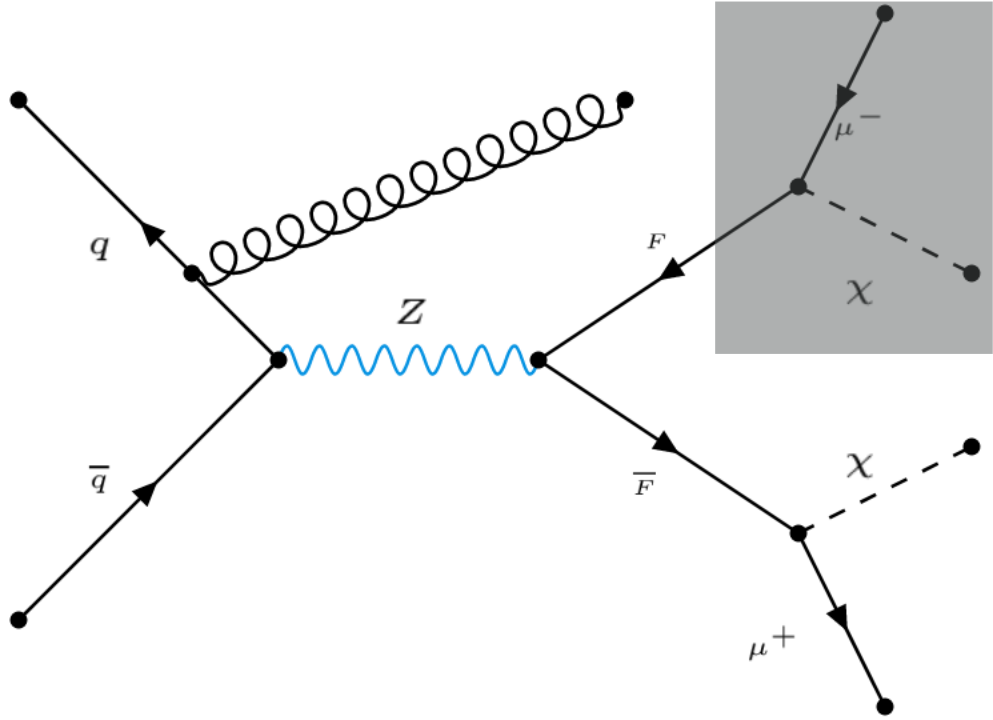
\includegraphics[width=0.45\textwidth]{pictures/DYVLFOneMuon}\label{fig6}
	\caption{{\scriptsize Pair-production of vector-like fermions, followed by their decay into a lepton and the DM particle, one missing lepton and a ISR jet }}
	
\end{figure}

\end{frame}

% ------------------------------------------------------------------------------------------------
\begin{frame}
\frametitle{Parameter Region}

\begin{figure}[!tbp]
	\centering
	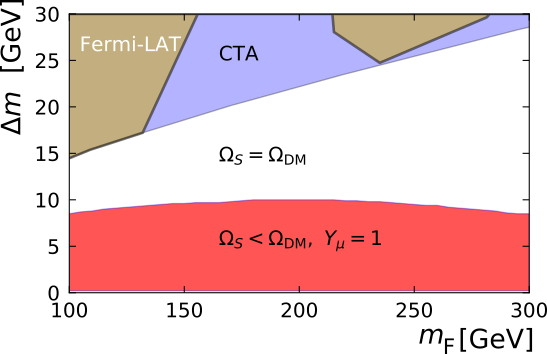
\includegraphics[width=0.9\textwidth]{pictures/PS}
	\caption{{\scriptsize $m_F$ vs $\Delta m$. The brown upper region is excluded by Fermi-LAT H.E.E.S, while the combined upper region with light and dark magenta are the prospects for Cherenkov Telescope Array. The Red area is the area where the relic density is not satisfy by the model}}
	\label{fig7}
\end{figure}


\end{frame}
% ------------------------------------------------------------------------------------------------
% ------------------------------------------------------------------------------------------------
\begin{frame}
\frametitle{Background}
The backgrounds for this process are single top, WZ, and w+jets. This last one being the most important.

\begin{figure}[!tbp]
	\centering
	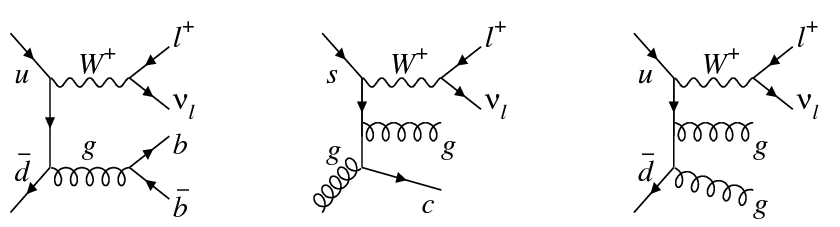
\includegraphics[width=0.9\textwidth]{pictures/WPlusJets}\label{fig8}
	\caption{{\small Some W+jets diagrams}}
	
\end{figure}

\end{frame}
% ------------------------------------------------------------------------------------------------
\begin{frame}
\section{Samples Generation}
\frametitle{Samples Generation}
\begin{justify}
	The Monte Carlo(MC) collision samples for the signal and the BackGrounds (BG) were generated using a combination of MadGraph (version 2.5.5 ) ~%\cite{Alwall2011} 
 for the event generation, Pythia (version 8.233)~  %\cite{Sjostrand:2014zea} 
for the hadronization and Delphes (version 3.4.1)~  %\cite{deFavereau:2013fsa} 
for the detector effect emulation.
\end{justify}
\begin{table}[]
	{\centering
		\begin{tabular}{llll}
			\hline
										& \textbf{W+Jets}	& \textbf{WZ}	& \textbf{SingleTop}	\\\hline
			$\sigma$ (Pb) 				& 3377.37    		& 22.82       	& 288.17     			\\
			$\sigma\times\mathcal{L}$   & 337737000   		& 2282000     	& 28817000   			\\
			MC            				& 50214     		& 173715      	& 319006      			\\
			Weight        				& 6725.95 			& 14.65 		& 90.33					\\\hline
		
		\end{tabular}
		
		\caption{Weights for the MC samples, based on the expected events.}
		\label{WeightsSamplesTable}
	}
\end{table}

\end{frame}

% ------------------------------------------------------------------------------------------------
% ------------------------------------------------------------------------------------------------

\begin{frame}
\frametitle{Background Tunig}
{\small To generate the background we use the tunes extract for the data from CMS at the reference [CMS-PAS-GEN-17-001] }

{\scriptsize
\begin{table}[]
	\begin{tabular}{ll}
		\hline
		\textbf{PYTHIA parameter}                & \textbf{Value} \\\hline
		PDF Set                                  & NNPDF3.1       \\
		$\alpha_S(MZ)$                           & 0.118          \\
		SPACESHOWER:RAPIDITYORDER                & on             \\
		MULTIPARTONINTERACTIONS:ECMREF {[}GeV{]} & 7000           \\
		$\alpha^{ISR}_S$                         & 0.118/NLO      \\
		$\alpha^{FSR}_S$                         & 0.118/NLO      \\
		$\alpha^{MPI}_S$                         & 0.118/NLO      \\
		$\alpha^{ME}_S$                          & 0.118/NLO      \\
		MULTIPARTONINTERACTIONS:PT0REF {[}GeV{]} & 1.41           \\
		MULTIPARTONINTERACTIONS:ECMPOW           & 0.03344        \\
		MULTIPARTONINTERACTIONS:CORERADIUS       & 0.7634         \\
		MULTIPARTONINTERACTIONS:COREFRACTION     & 0.63           \\
		COLORRECONNECTION:RANGE                  & 5.176          \\
		$\chi^2/dof$                             & 1.04           \\\hline
	\end{tabular}
		\caption{Pythia 8 parameter values }
		\label{PythiaTune}

\end{table}
}

\end{frame}

% ------------------------------------------------------------------------------------------------
% ------------------------------------------------------------------------------------------------

\begin{frame}
\frametitle{Background Tuning}
After the tunig we use Rivet[] over the analysis [PhysRevD.96.072005] to compare 

\begin{figure}[!h]

	\begin{subfigure}[b]{0.44\textwidth}
		\centering
		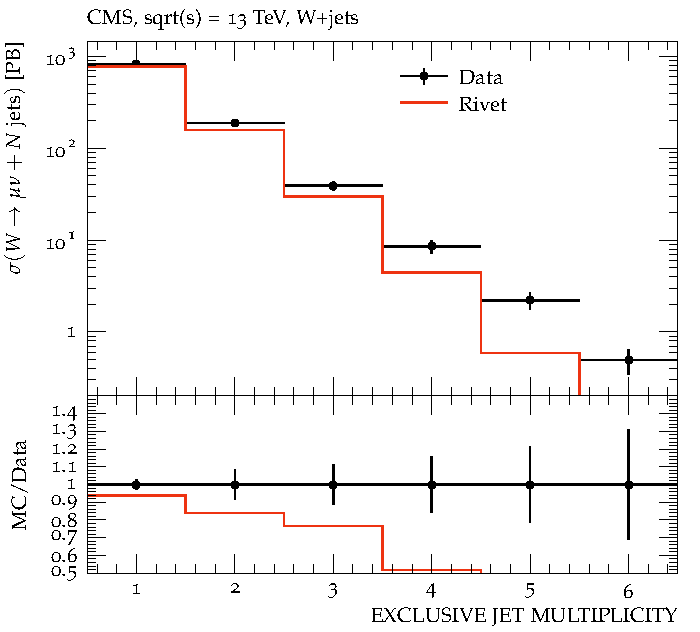
\includegraphics[width=\textwidth]{pictures/MCTunig/EXCLUSIVE_JET_MULTIPLICITY}
		\caption{\label{EXCLUSIVE_JET_MULTIPLICITYTune}}
	\end{subfigure}
	\begin{subfigure}[b]{0.44\textwidth}
		\centering
		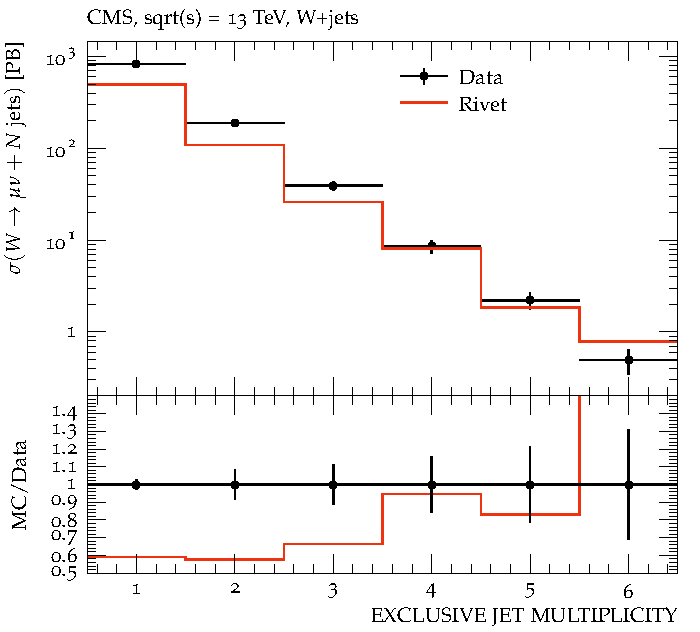
\includegraphics[width=\textwidth]{pictures/MCTunig/EXCLUSIVE_JET_MULTIPLICITY_Nelson}
		\caption{\label{EXCLUSIVE_JET_MULTIPLICITY}}
	\end{subfigure}
	\caption{ \justifying{ Differential cross section measurement for the exclusive jet multiplicities with tune (\subref{EXCLUSIVE_JET_MULTIPLICITYTune}) and with out tune (\subref{EXCLUSIVE_JET_MULTIPLICITY})} }
\end{figure}


\end{frame}

% ------------------------------------------------------------------------------------------------
% ------------------------------------------------------------------------------------------------

\begin{frame}
\frametitle{Background Tuning}
 

\begin{figure}[!h]
	
	\begin{subfigure}[b]{0.44\textwidth}
		\centering
		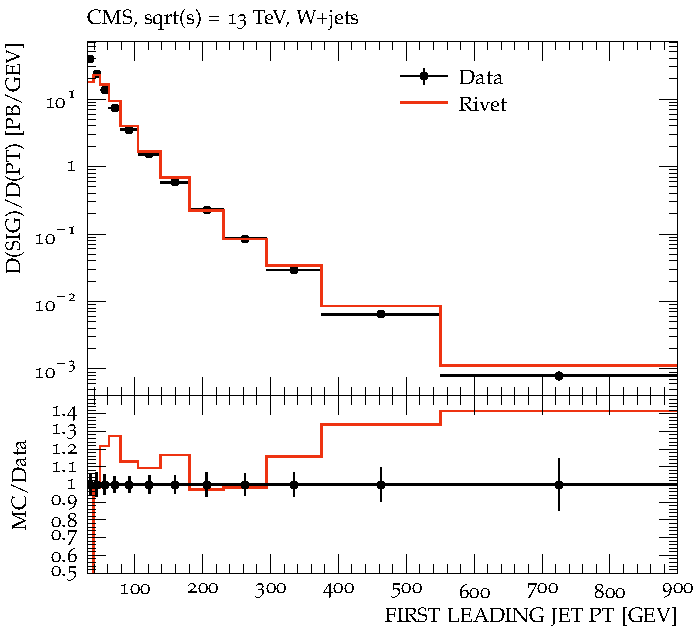
\includegraphics[width=\textwidth]{pictures/MCTunig/FIRST_LEADING_JET_PT}
		\caption{\label{FIRST_LEADING_JET_PTTune}}
	\end{subfigure}
	\begin{subfigure}[b]{0.44\textwidth}
		\centering
		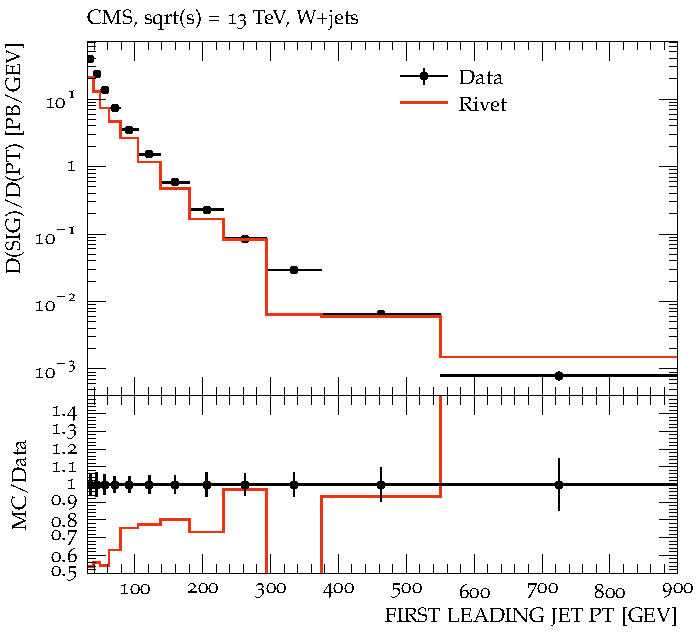
\includegraphics[width=\textwidth]{pictures/MCTunig/FIRST_LEADING_JET_PT_Nelson}
		\caption{\label{FIRST_LEADING_JET_PT}}
	\end{subfigure}
	\caption{ \justifying{ Differential cross section measurement for the exclusive jet multiplicities with tune (\subref{FIRST_LEADING_JET_PTTune}) and with out tune (\subref{FIRST_LEADING_JET_PT})} }
\end{figure}


\end{frame}

% ------------------------------------------------------------------------------------------------
% ------------------------------------------------------------------------------------------------

\begin{frame}
\frametitle{Background Tuning}

\begin{figure}[!h]
	
	\begin{subfigure}[b]{0.44\textwidth}
		\centering
		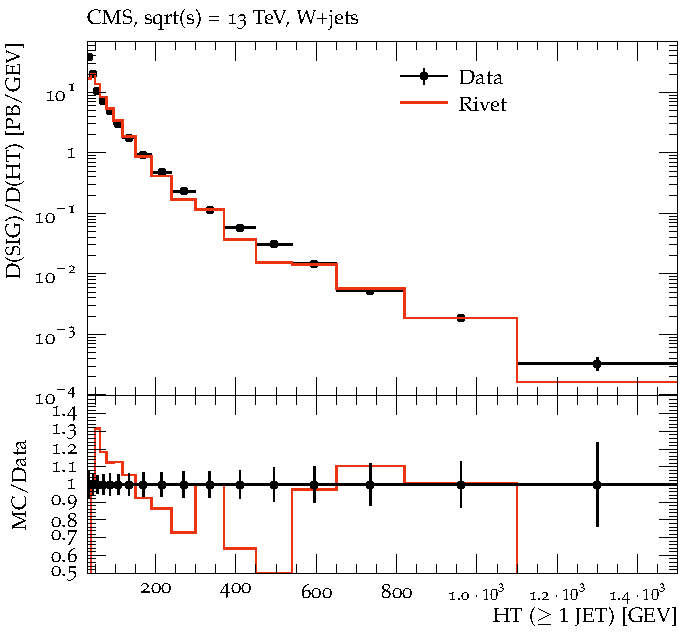
\includegraphics[width=\textwidth]{pictures/MCTunig/HT}
		\caption{\label{HTTune}}
	\end{subfigure}
	\begin{subfigure}[b]{0.44\textwidth}
		\centering
		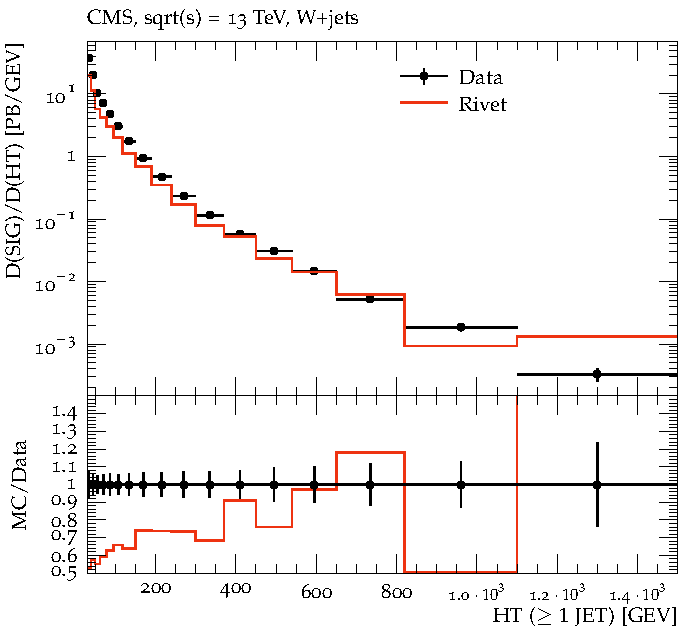
\includegraphics[width=\textwidth]{pictures/MCTunig/HT_Nelson}
		\caption{\label{HT}}
	\end{subfigure}
	\caption{ \justifying{ Differential cross section measurement for the jets HT for at least 1 jet with tune (\subref{HTTune}) and with out tune (\subref{HT})} }
\end{figure}


\end{frame}

% ------------------------------------------------------------------------------------------------
% ------------------------------------------------------------------------------------------------

\begin{frame}
\section{Samples Selection}
\frametitle{Selection}
The values for the cuts were defined through an optimization process based on the $\frac{S}{\sqrt{S+B}}$, we normalize all MC to $100~\text{fb}^{-1}$ luminosity and the
signal mass point  $m_{F}=140$GeV vs  $\Delta m=20$GeV



\begin{figure}[!h]
	
	\centering
	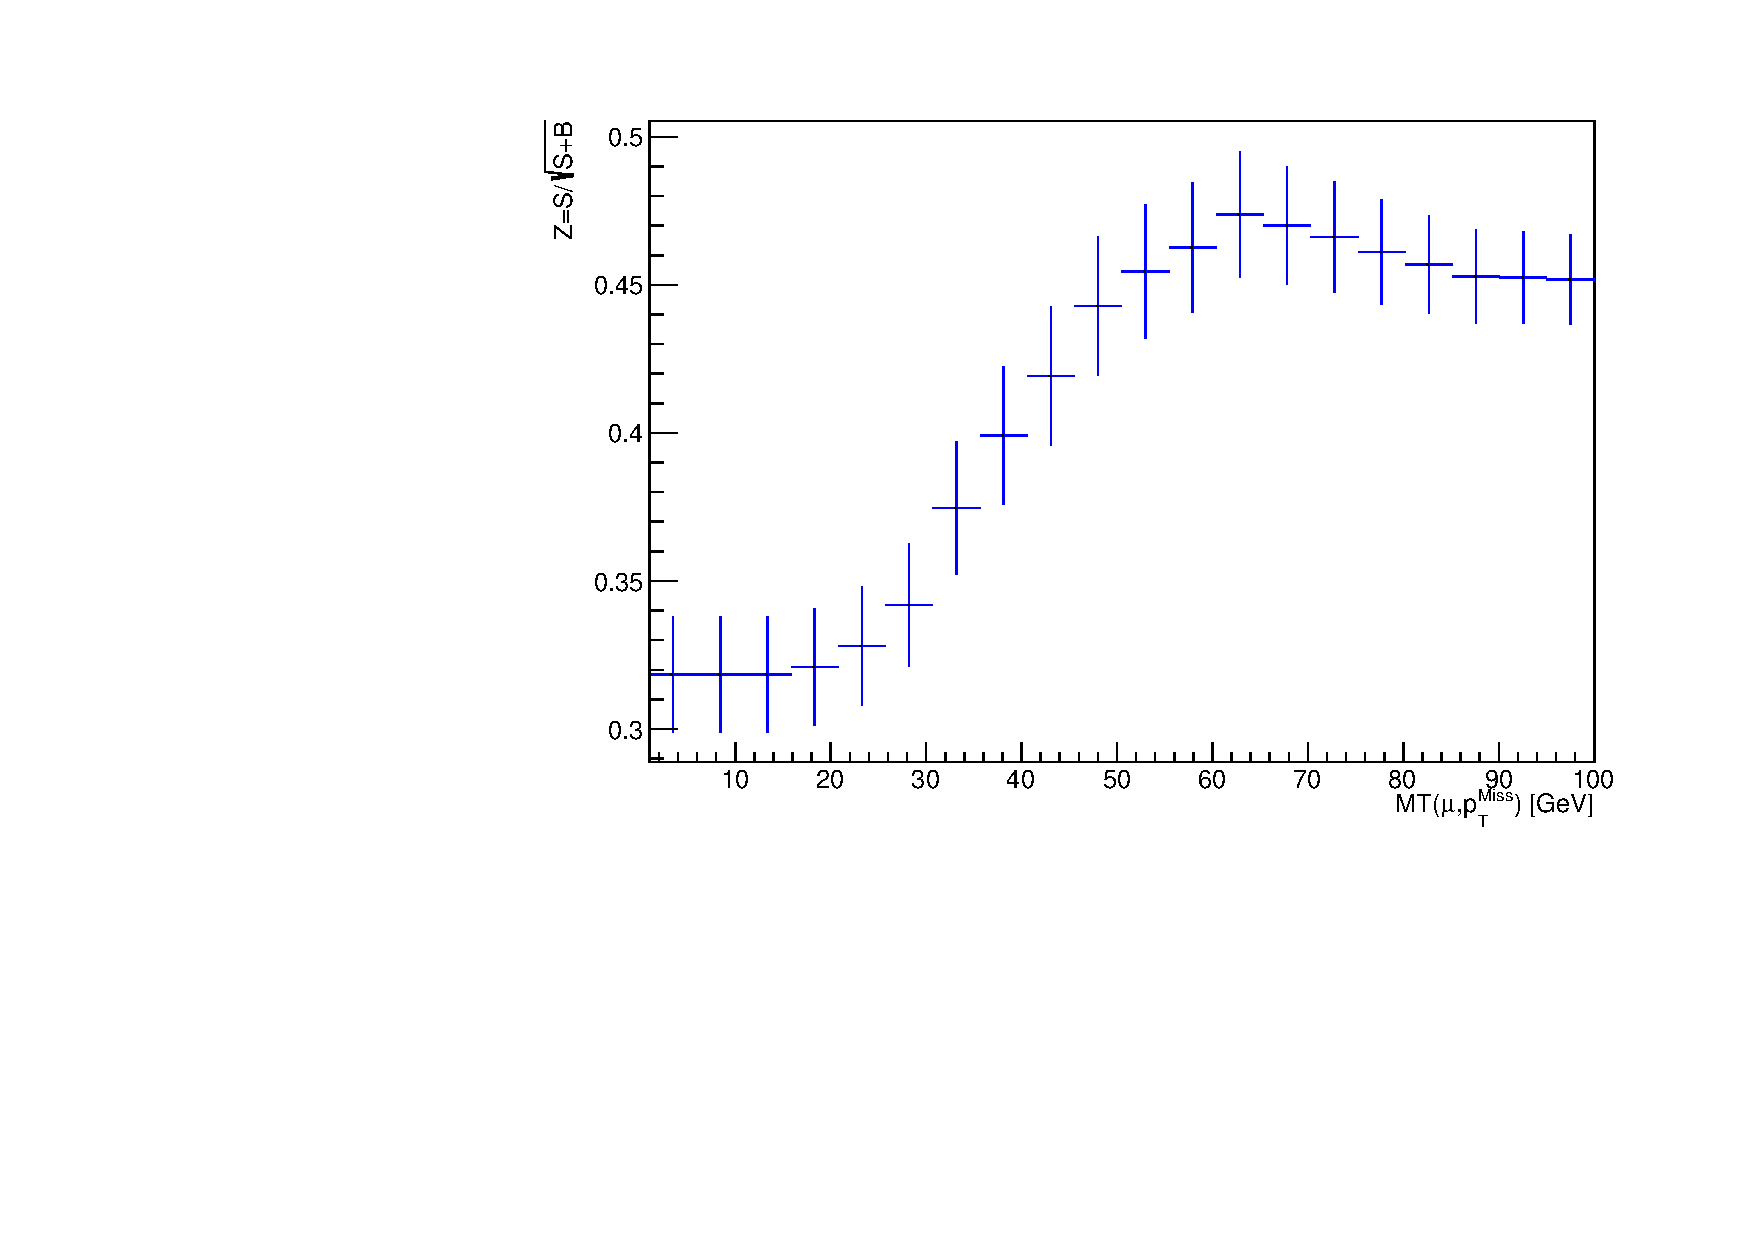
\includegraphics[scale=0.45]{pictures/Selection/SigLT_MT}
	\caption{Significance of the cut (type less-
		than) for $m_T(\mu,p_{T}^{Miss}$ \label{}}
	
\end{figure}


\end{frame}

% ------------------------------------------------------------------------------------------------
% ------------------------------------------------------------------------------------------------

\begin{frame}
\section{Samples Selection}
\frametitle{Selection}


\begin{figure}[!h]
	
	\centering
	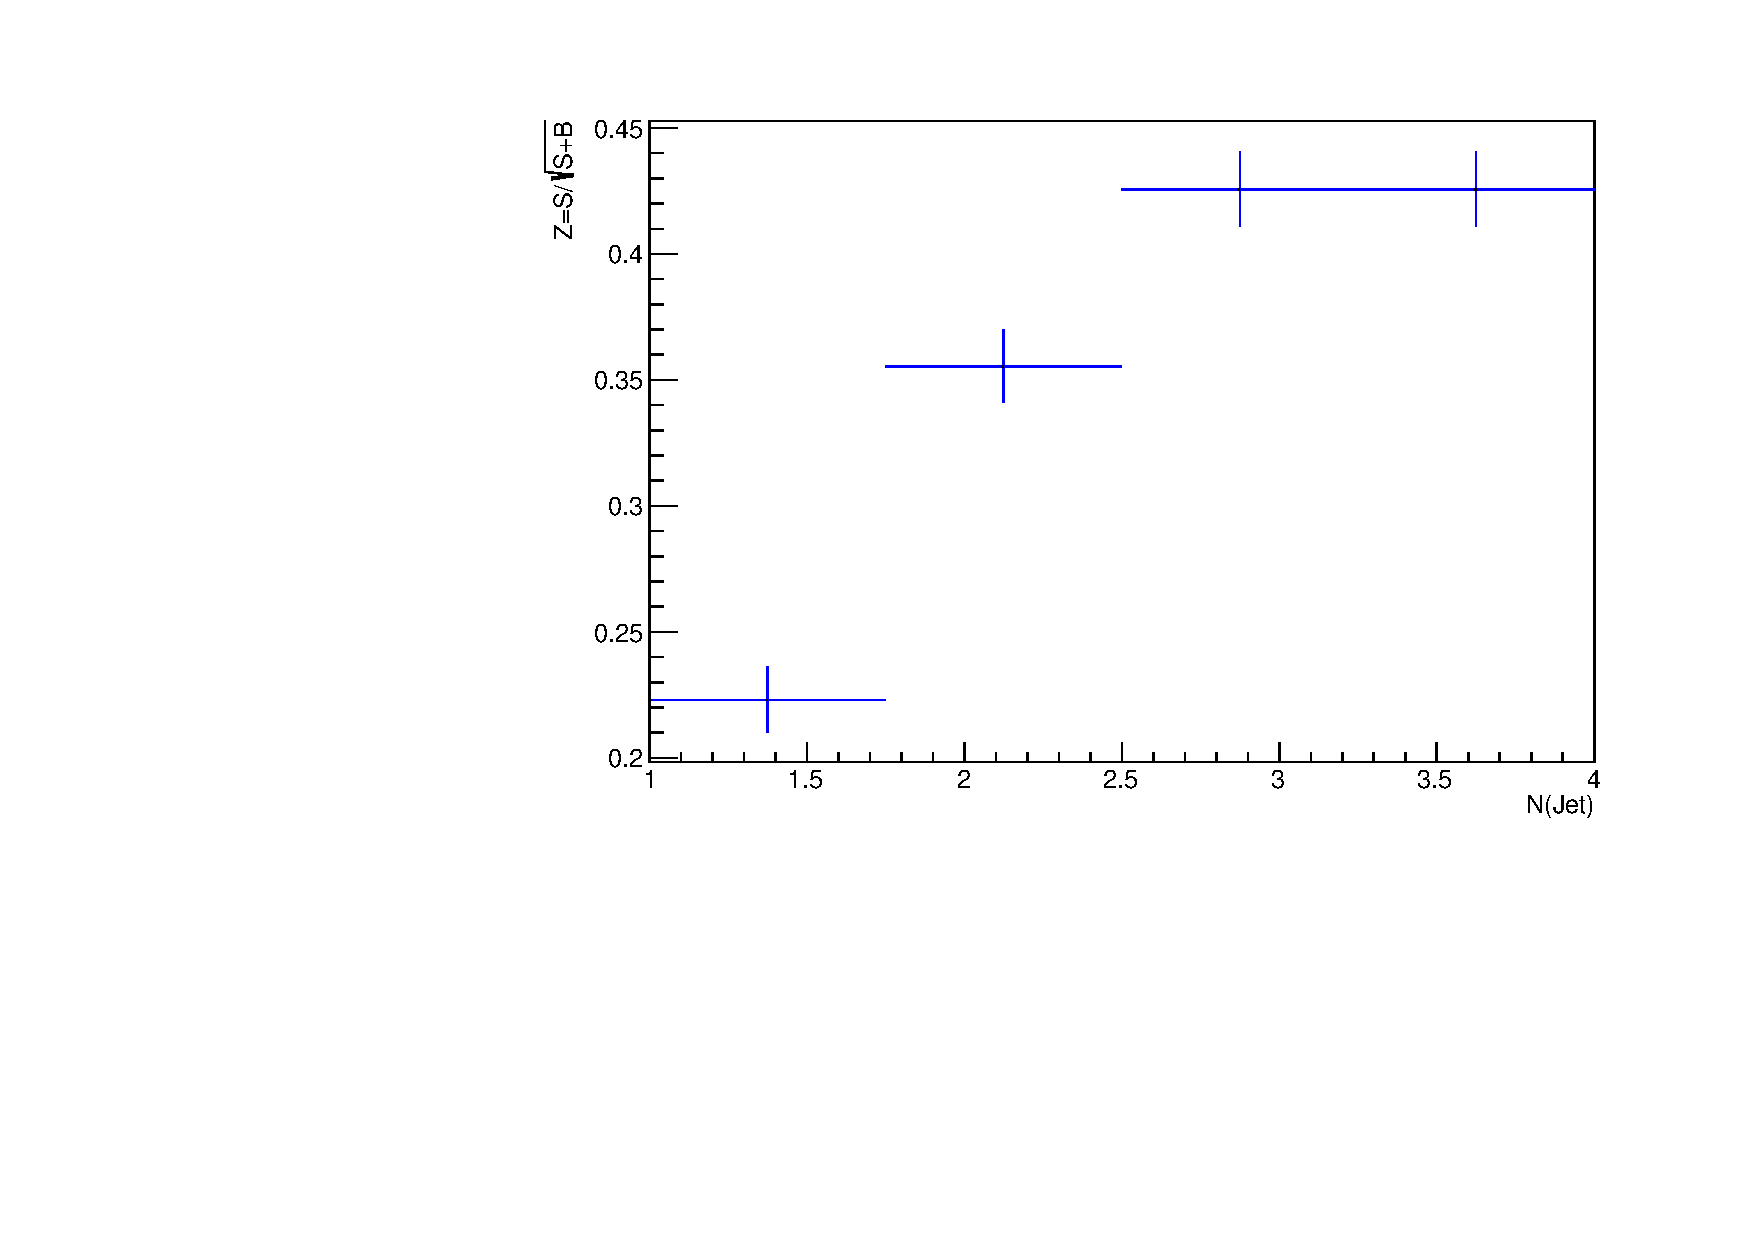
\includegraphics[scale=0.45]{pictures/Selection/SigLT_NJet}
	\caption{ Significance of the cut (type less-
		than) for the number of Jets\label{}}
	
\end{figure}


\end{frame}

% ------------------------------------------------------------------------------------------------
% ------------------------------------------------------------------------------------------------

\begin{frame}
\section{Samples Selection}
\frametitle{Selection}


\begin{figure}[!h]
	
\centering
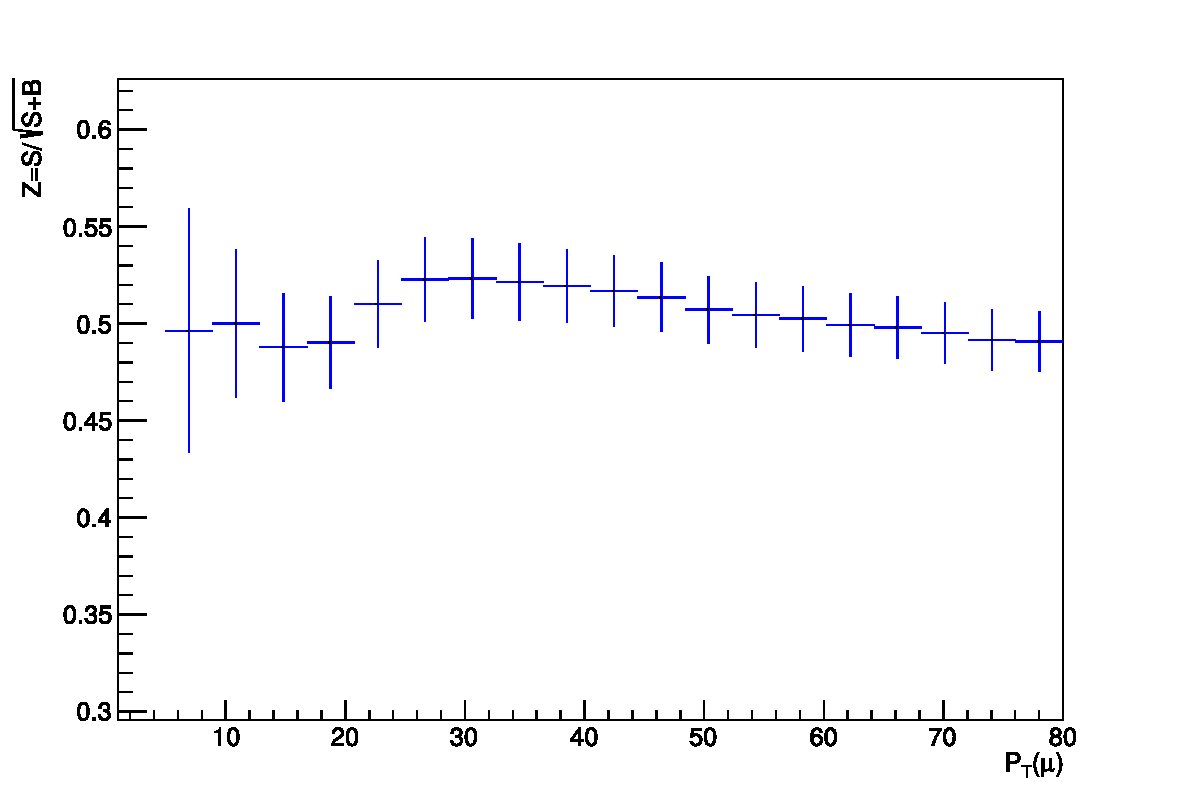
\includegraphics[scale=0.45]{pictures/Selection/SigLT_P_Tmu}
\caption{Significance of the cut (type less-
	than) for the $p_T(\mu)$\label{}}

\end{figure}


\end{frame}

% ------------------------------------------------------------------------------------------------
\begin{frame}

\frametitle{Selection}


\begin{table}[]
	{\centering
		\begin{tabular}{ll}
			\hline
			\textbf{Cut}                       & \textbf{Selection}                                           \\\hline
			Trigger                            & MonoJet  \\
			$N(\mu)$                           & 1                                                            \\
			$p_T(\mu)$                         & \textless{}30 GeV                                            \\
			$N(Jet)$                           & \textless{}3                                                 \\
			%$p_T(LeadingJet)$                  & \textless{}20                                                \\
			m\_T(p\_T(\textbackslash{}mu),MET) & \textless{}60                                             \\ \hline
		\end{tabular}
		
		\caption{Cuts, monoJet triggers means MET\textgreater{}110 GeV, MHT\textgreater{}110 GeV}
		\label{CutsTable}
	}
\end{table}



\end{frame}

% ------------------------------------------------------------------------------------------------
\begin{frame}
\frametitle{Results}

\begin{figure}
	\centering
	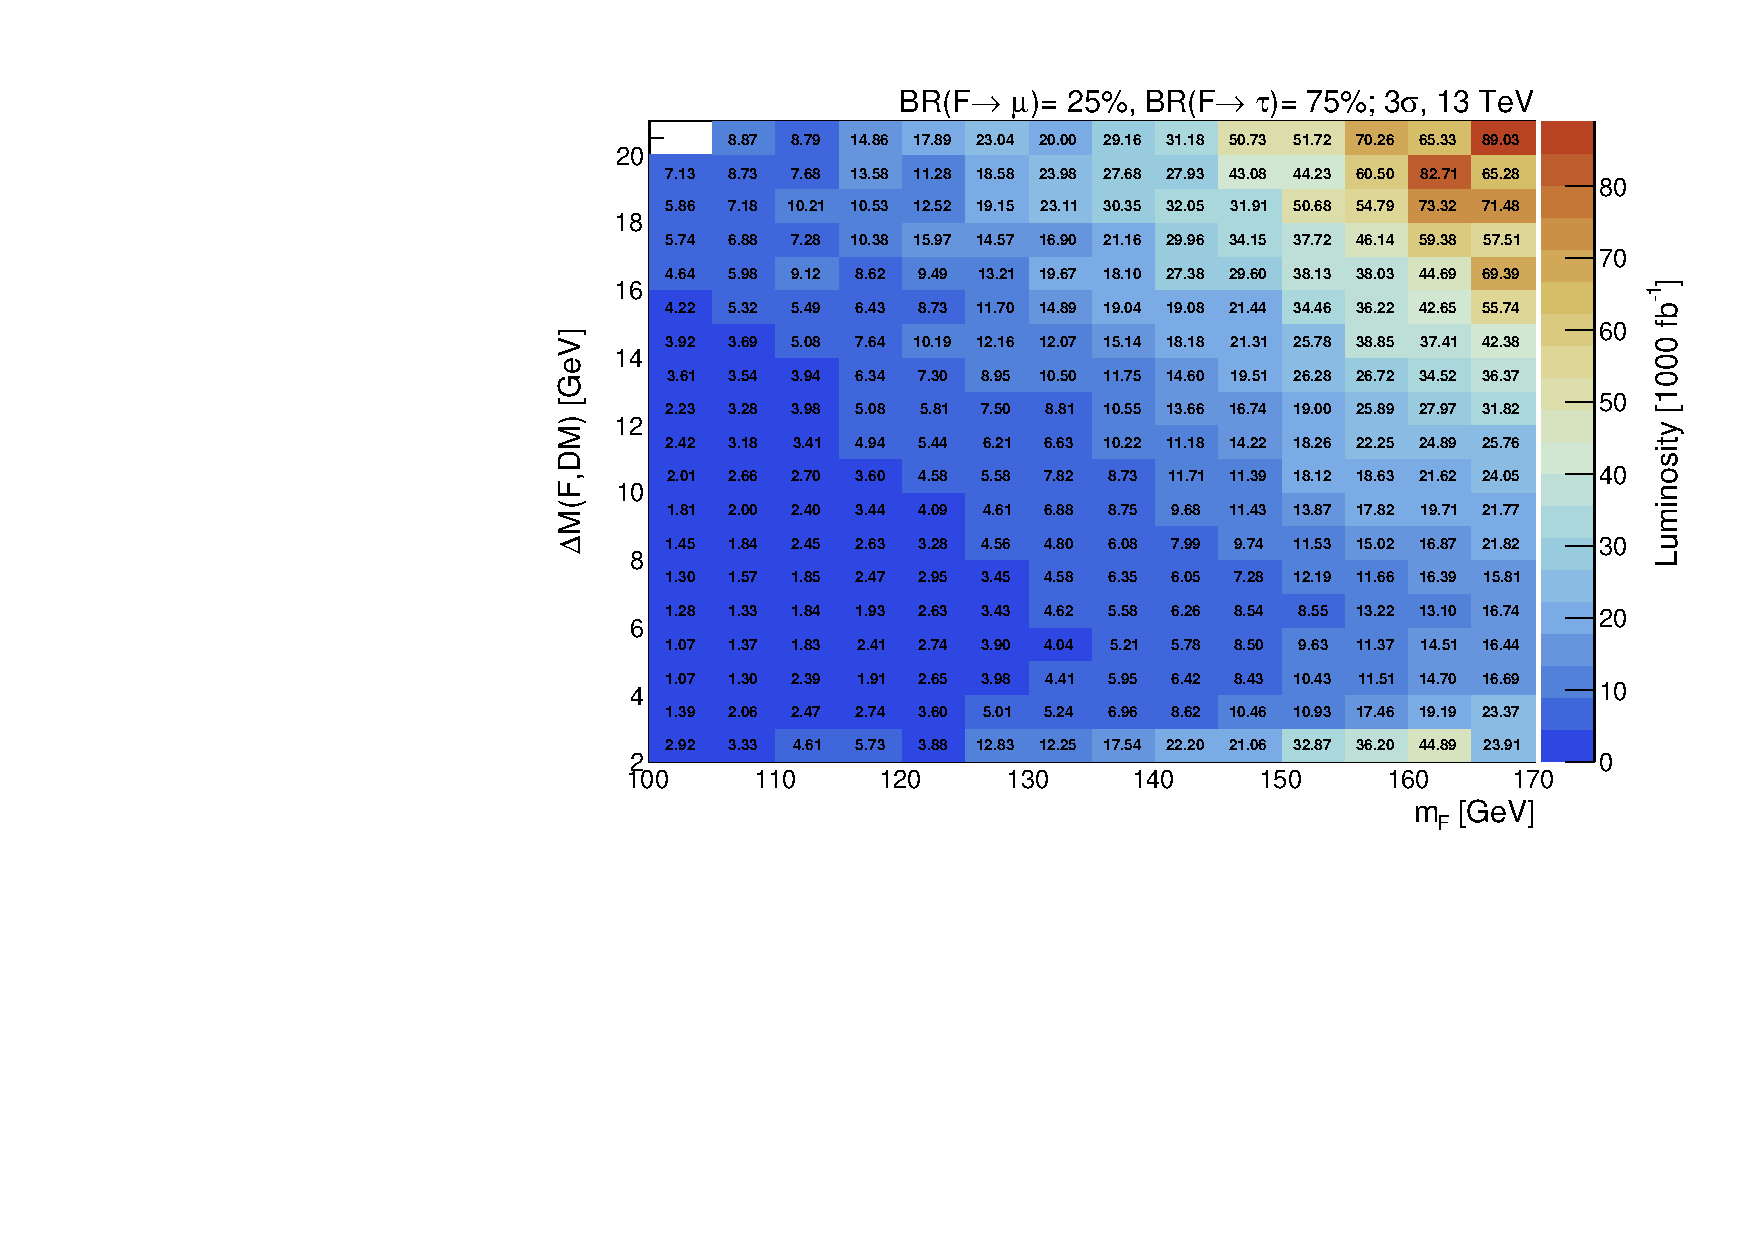
\includegraphics[scale=0.45]{pictures/LumiToExclusionSigma3_BRmu25tau75} 
	\caption{3 $\sigma$ reach for $m_{F}$ vs  $\Delta m$ parameter space for various luminosity in $1000\text{fb}^{-1}$. }
	\label{results}
\end{figure}

\end{frame}

% ------------------------------------------------------------------------------------------------
% ------------------------------------------------------------------------------------------------

\begin{frame}
\frametitle{Exclusion Potential}

We want to exclude the region of parameters of the model, which is still unexplored Figure \ref{fig7}, the intersection between the regions in Figures \ref{fig7} and \ref{results} shows the exclusion potential for the study.
The exclusion is carried out assuming that what is going to be observed is only the standard model

\end{frame}

% ------------------------------------------------------------------------------------------------
% ------------------------------------------------------------------------------------------------

\section{Remarks}
\begin{frame}
\frametitle{Remarks}

\begin{exampleblock}{}
	
	\begin{enumerate}

		\item Although the model have been analyzed. there is still the region of the parameter space ($\Delta m=m_{F}-m_S\lesssim 50\ \text{GeV}$) with exclusion potential.
		\item The full dark matter content may be explained either by freeze-out at higher redshifts, or by another dark matter content.
		\item  We can obtain exclusion sensitivity over a large region of parameter has not yet been covered by any other search.
	\end{enumerate}

\end{exampleblock}

\end{frame}
% ------------------------------------------------------------------------------------------------



% ------------------------------------------------------------------------------------------------

\ThankYouFrame

% ------------------------------------------------------------------------------------------------
% ------------------------------------------------------------------------------------------------
\section{Backup}
\begin{frame}
\frametitle{MC Validation}
{\justifying
To validate the W+Jets background we use the Table 1 from [CMS-PAS-SMP-16-005], where they have ${\sqrt{s}=13}$ TeV proton-proton MC samples normalized to an
integrated luminosity of 2.5 $ \text{fb}^{-1}$
}
\begin{table}[]
	\resizebox{\textwidth}{!}{\begin{tabular}{lllll}
	
		\hline
		& $N_{Jets}=1$ & $N_{Jets}=2$ & $N_{Jets}=3$ & $N_{Jets}=4$ \\\hline
		CMS-PAS-SMP-16-005 & 1854568      & 384856       & 78271        & 14577        \\
		VLF-study          & 370200       & 345520       & 137282       & 62471        \\
		Diff               & 1484368      & 39336        & -59011       & -47894      \\\hline
	
	\end{tabular}}
	\caption{{\scriptsize  Number of events simulation as a function of the exclusive jet multiplicity. Events are required to have exactly one muon and one or more jets for the $W \rightarrow \mu\nu +jets$ production, muons are required to have $p_T > 25$ GeV and $|\eta| < 2.4$, and jets are required to have $p_T > 30$ GeV, and last $M_T > 50$ GeV}}
\end{table}

Currently looking into it.

\end{frame}




% ------------------------------------------------------------------------------------------------
\begin{frame}
\frametitle{Relation with Fermi LAT}

Gamma-ray from the Galactic center measured Fermi-LAT Collaboration could be explained by these type of models.

\begin{figure}
	\centering
	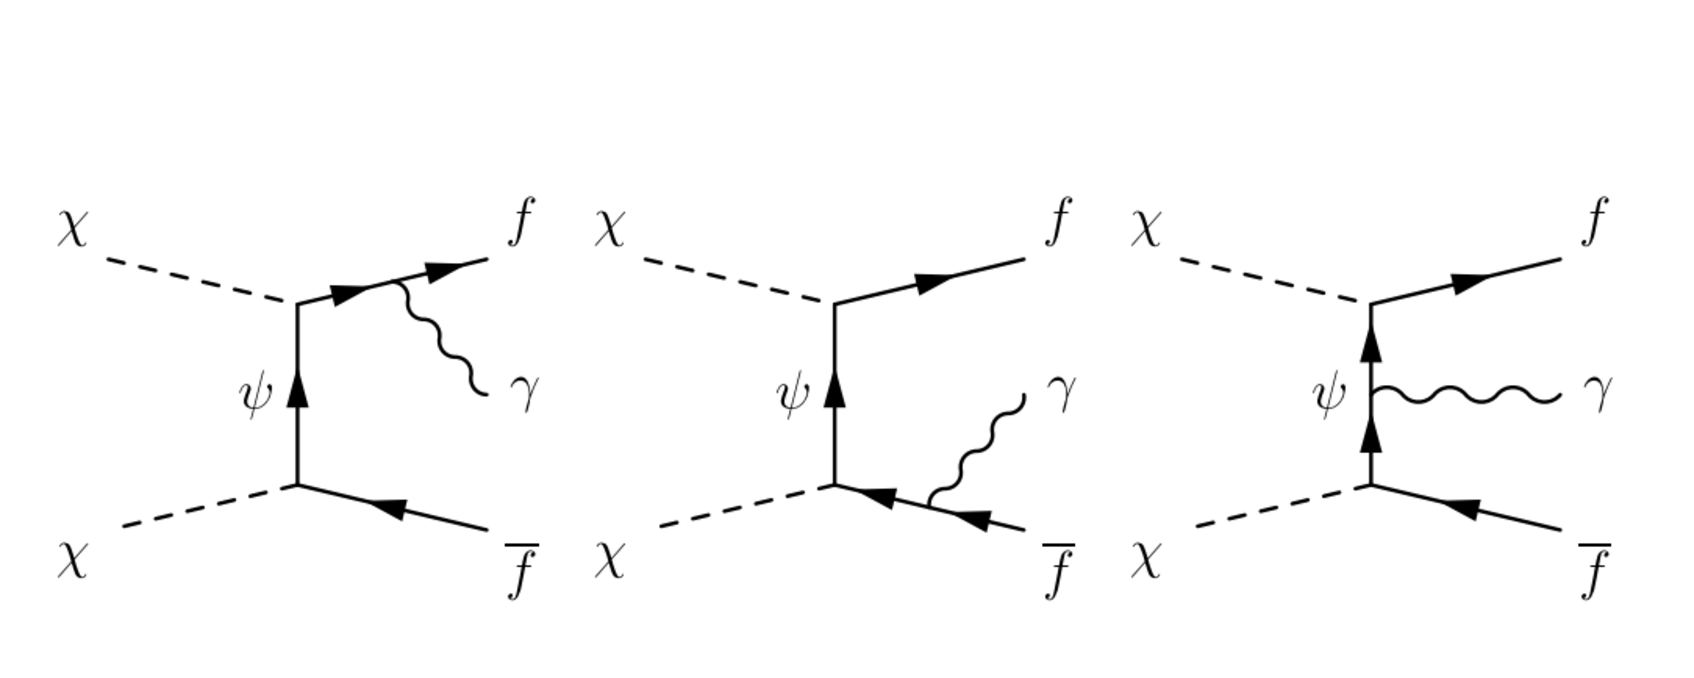
\includegraphics[scale=0.3]{pictures/Bremsstrahlung} 
	\caption{Internal Bremsstrahlung processes of (real) scalar DM. From [Phys Rev Lett. 2013 Aug 30;111(9):091301.] }
	\label{fig:Brem}
\end{figure}

\end{frame}
% ------------------------------------------------------------------------------------------------

% ------------------------------------------------------------------------------------------------
\begin{frame}
\frametitle{Similar Searches}
{\footnotesize
\begin{itemize}
	\item Search for top squark pair production in pp collisions at $sqrt(s) = 13$ TeV using single lepton events (arXiv:1706.04402) \ref{04402}
	\item Search for top squarks decaying via four-body or chargino-mediated modes in single-lepton final states in proton-proton collisions at $sqrt(s) = 13$ TeV (arXiv:1805.05784)
	
\end{itemize}
}
\begin{figure}
	\centering
	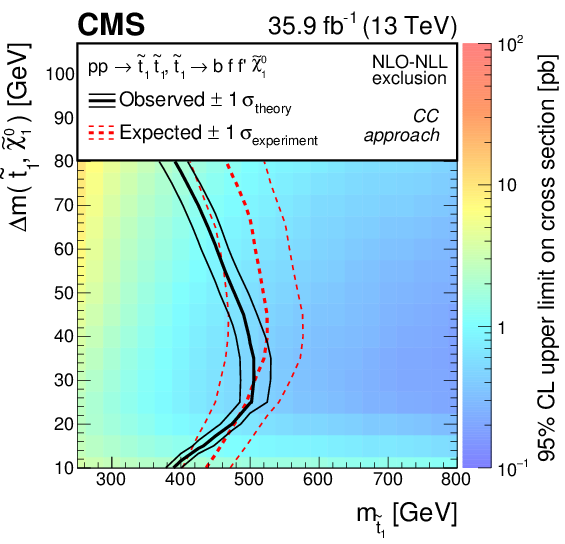
\includegraphics[scale=0.2]{pictures/Figure_007-a} 
	\caption{{\scriptsize 	Exclusion limit at 95\% for the four-body decay of the top squark as a function of $m(\tilde{t})$ and $\delta m$ } }
	\label{04402}
\end{figure}

\end{frame}
% ------------------------------------------------------------------------------------------------



% ------------------------------------------------------------------------------------------------

%\begin{frame}
%\frametitle{M}

%\end{frame}

% ------------------------------------------------------------------------------------------------

% ------------------------------------------------------------------------------------------------

% ------------------------------------------------------------------------------------------------

%\section{Bibliography}
%\begin{frame}{Bibliography}
%\frametitle{Bibliography}

%\bibliographystyle{apalike}
%\bibliography{references}
%\end{frame}

% ------------------------------------------------------------------------------------------------
\end{document}
